\documentclass[online,a4paper]{isw}

%% Fill in your thesis' data here
% @todo Make sure that capitalized words will appear capitalized in the final document, too
%\title{This Shall be a Great Thesis Paper with an Extremely Long Title but who Cares}
%\subtitle{Some theses even have subtitles}
%\date{2015-08-28}
%\author{Maschinen Bauer}
%\matriculation{1234567}
%\examiner{Jun.-Prof.~Dr.-Ing.~Andreas Pott}
%\major{Technische Kybernetik}
%\supervisor{Dipl.-Ing.~Philipp Tempel \and Dipl.-Ing.~Martin Wehr}
%\partner{Fraunhofer IPA}
%\renewcommand{\partnerlogo}{images/logo/simtech}


\title{This Shall be a Great Thesis Paper with an Extremely Long Title but who Cares because it is just an exemplary title}
\subtitle{Some Theses Even Have Subtitles Which Should Not be as Long as This Subtitle Is Because it is too Long}
\author{Maschinen Bauer}
\major{Mechatronik}
\examiner{Jun.-Prof.~Dr.-Ing.~Andreas Pott}
\supervisor{Dipl.-Ing.~Philipp Tempel \and Dipl.-Ing.~Martin Wehr}
\matriculation{1234567}
\date{2015-08-28}

\usepackage{lipsum}



% And done with the configuration you are!

\usepackage{lipsum}

\begin{document}
    % Sets the pagestyle properly, sets roman page numbers, etc
    \frontmatter
    
    % Creates the title page
    \maketitle
    
    % Creates a German titlepage (if you don't issue the \title - and possibly the subtitle - command inside this environment, the main language's title - and subtitle - will be displayed)
    \begin{otherlanguage}{ngerman}
        % @TODO If we change the name of the university here, it will stick to this for the remainder of the file (which is not what we want, so we need to find a way to fix this and set localization based on the currently active language)
        \university{Universtit\"at Stuttgart}
        \title{Dies soll ein langer Titel der Arbeit sein damit er extra lang ist aber das macht ja niemandem etwas aus}
        \subtitle{Manche Arbeiten haben sogar Untertitel}
        \maketitle
    \end{otherlanguage}
    
    % Add a dedication (if you want to)
%    \begin{dedication}
%        \lipsum
%    \end{dedication}
    
    % Add declaration of authorship (MUST be signed in version printed and handed in)
%    \DeclarationOfAuthorship
    
    % Create the thesis abstract
    \begin{thesisabstract}
        \lipsum
        \keywords{a, list, of, keywords}
    \end{thesisabstract}
    
    \begin{otherlanguage}{ngerman}
        \begin{thesisabstract}
            \lipsum
        \end{thesisabstract}
    \end{otherlanguage}
    
    %% Output all the different "list of "
    % Table of contents
    \tableofcontents
    % List of all figures
    \listoffigures
    % List of all tables
    \listoftables
    % List of all used mathematical symbols
    % @todo Add some glossary package
%    \printglossaries
    
    % List of all abbreviations
    % @todo Add some nomenclature package
%    \printnomenclature
    
    % List of open todos (finally and only in "draft" mode)
%    \listoftodos
    
    % Switch back to arabic page numbering and proper page headers and footers
    \mainmatter
    
    %%% This is where your main content will go
    \lstset{language=[LaTeX]TeX}

\chapter{User Documentation}

\begin{intro}
In this chapter, the user will get a general introduction to using the thesis template and will be enabled to start his/her work.
Further information is given in the subsequent chapters.
But don't be afraid, there is no need for you to read through all of it before starting your work.
Instead, you might find it useful to just look at the table of contents and decide which sections you need to look at later when looking for a solution to a problem.
\end{intro}


\section{Introduction}\label{sec:user-documentation:introduction}

\subsection{Target Users}\label{sec:user-documentation:target-users}

Writing a good thesis can be cumbersome if you have never done it before.
Even for experienced researches having published a sum of papers, writing up a thesis is not the same.
Without underestimating the complexity of writing a thesis, it is cumbersome to get it all nicely wrapped up and in layout that is consistent from start to end.
This thesis template tries to fill the gap between content and layout by providing you with certain commonly used packages and styles set to have a consistent layout that you don't have to bother about maintaining.


\subsection{Features of the Class}\label{sec:user-documentation:features}

With this thesis template you write a simple, nicely typeset thesis without the hassle of needing to configure it such that it suits the needs of your department (it should have applied all the necessary style guidelines already).


\subsection{How to Get Started}\label{sec:user-documentation:get-started}

In order to get your thesis started, there is a few things necessary to set up.
One of them being obviously the choice of a good typewriting environment.
The list out there for writing your thesis is longer than it should be so we will just briefly mention some of the most common editors (both IDE and simple text editors).
Choose by your own needs


\subsubsection{Configure Editor and System Settings}\label{sec:user-documentation:configure-system}

You must choose a \LaTeX distribution and an editor.
For a list of editors, please refer to or the following list (which is only an excerpt from the SO page).
We prefer TeXstudio even though its implementation of using some keys can be cumbersome at times.

\paragraph{Emacs with AUCTeX}

\begin{itemize}
    \item \textit{Platforms:} Windows, Mac (incl. Aquamacs fork), Unix
    \item \textit{License:} Free software (GPL)
    \item \textit{Languages:} de, dk, fr, is, it, jp, nl, pl, se, sk are supported by AUCTeX language styles
    \item \textit{Unicode:} Yes, from Emacs 23, characters are represented using Unicode
    \item \textit{RTL/bidirectional support:} From Emacs 24, through bidi-mode
    \item \textit{\% !TEX directives:} No, but has several realizations of file local variables
    \item \textit{Syntax highlighting:} Yes, customisable through customize and Elisp
    \item \textit{Code completion:} Yes, via Emacs Predictive Completion, which supports AUCTeX without further configuration
    \item \textit{Code folding:} Yes
    \item \textit{Spell checking:} Yes
    \item \textit{SyncTeX:} Yes
    \item \textit{Built-in output viewer:} Yes
    \item \textit{Project management:} org-mode, reftex-mode, speedbar
\end{itemize}

\paragraph{Vim with LaTeX-suite}

\begin{itemize}
    \item \textit{Platforms:} Windows, Mac, Linux and others
    \item \textit{License:} Open Source Charityware
    \item \textit{Languages:} ?
    \item \textit{Unicode:} Yes
    \item \textit{RTL/bidi support:} partially
    \item \textit{\% !TEX directives:} No, but has modelines
    \item \textit{Syntax Highlighting:} Yes, customizable
    \item \textit{Code Completion:} Yes (using Omni Completion, extendable with SnipMate plugin)
    \item \textit{Code Folding:} Yes
    \item \textit{Spell Checking:} Yes
    \item \textit{SyncTeX:} Yes, see e.g. this question
    \item \textit{Built-in Output Viewer:} No
    \item \textit{Project Management:} ?
\end{itemize}

\paragraph{Texmaker}

\begin{itemize}
    \item \textit{Platforms:} Windows XP/Vista/7/8, OS X 10.5+, Linux
    \item \textit{License:} GPL license, free
    \item \textit{Languages:} cs, de, el, en, es, fa, fr, gl, hu, it, nl, pl, pt, pt (bra), ru, se, sr, zh (cn), zh (tw)
    \item \textit{Unicode:} Yes
    \item \textit{RTL/bidi:} ?
    \item \textit{\% !TEX directives:} No
    \item \textit{Syntax Highlighting:} Yes, customizable
    \item \textit{Code Completion:} Yes, customizable
    \item \textit{Code Folding:} Yes
    \item \textit{Spell Checking:} Yes
    \item \textit{SyncTeX:} Yes
    \item \textit{Built-in Output Viewer:} Yes, supports PDF
    \item \textit{Project Management:} Yes
\end{itemize}

\paragraph{TeXstudio (formerly TexMakerX)}

\begin{itemize}
    \item \textit{Platforms:} Windows XP/Vista/7, OS X, Linux, FreeBSD
    \item \textit{License:} GPL v2
    \item \textit{Languages:} cs, de, en, es, fr, hu, ja, pt\_BR, zh\_CN
    \item \textit{Unicode:} Yes
    \item \textit{RTL/bidi:} ?
    \item \textit{\% !TeX directives:} Yes
    \item \textit{Syntax Highlighting:} Yes, customizable
    \item \textit{Code Completion:} Yes, customizable and auto-customized
    \item \textit{Code Folding:} Yes
    \item \textit{Spell Checking:} Yes
    \item \textit{SyncTeX:} Yes
    \item \textit{Built-in Output Viewer:} Yes, supports PDF
    \item \textit{Project Management:} Yes
\end{itemize}

\paragraph{TeXworks}

\begin{itemize}
    \item \textit{Platforms:} Windows XP/Vista/7/8, OS X, Linux all pre-compiled plus source available
    \item \textit{License:} GPL
    \item \textit{Languages:} en, af, ar, ca, cs, de, fa, fo fr, it, ja, nl, ko, pl, pl, ru, sl, tr zh
    \item \textit{Unicode:} Yes
    \item \textit{RTL/bidi:} Yes
    \item \textit{\% !TEX directives:} Yes
    \item \textit{Syntax Highlighting:} Yes, regex-based
    \item \textit{Code Completion:} Yes, customizable based on 'known entry' list
    \item \textit{Code Folding:} No
    \item \textit{Spell Checking:} Yes, but have to install by hand
    \item \textit{SyncTeX:} Yes
    \item \textit{Built-in Output Viewer:} Yes, PDF (Poppler-based)
    \item \textit{Project Management:} No
\end{itemize}

\paragraph{TeXnicCenter}

\begin{itemize}
    \item \textit{Platforms:} Windows XP/Vista/7/8
    \item \textit{License:} Open Source
    \item \textit{Languages:} English, German, more dictionaries for spelling control downloadable
    \item \textit{Unicode:} Yes (in version 2, which was released mid-september 2013).
    \item \textit{RTL/bidi:} ?
    \item \textit{\% !TEX directives:} No
    \item \textit{Syntax Highlighting:} Yes, customizable (also background colour)
    \item \textit{Code Completion:} Yes
    \item \textit{Code Folding:} Yes
    \item \textit{Spell Checking:} Yes
    \item \textit{SyncTeX:} Yes
    \item \textit{Built-in Output Viewer:} No. You can config TeXnicCenter to use an external PDF viewer like Acrobat Reader or SumatraPDF with synchronized viewing.
    \item \textit{Project Management:} Yes
\end{itemize}

\subsubsection{Configuring the Document}\label{sec:user-documentation:configure-document}

Configuring your document to work should be quite easy.
Once you open the file given to you by your supervisor (\texttt{thesis.tex}) you will find some pre-defined values for the documentclass.
These need not be changed before you are actually submitting your thesis.
Further down you will find several commented commands, namely

\begin{itemize}
    \item \texttt{\textbackslash title\{\}} Your thesis title as chosen by you and your advisor.
    \item \texttt{\textbackslash subtitle\{\}} Theses may also have subtitles which can be set using this command.
    \item \texttt{\textbackslash date\{\}} The date that you will be handing in your thesis.
    \item \texttt{\textbackslash author\{\}} Your name. Obvious, right?
    \item \texttt{\textbackslash matriculation\{\}} Your matriculation identification.
    \item \texttt{\textbackslash examiner\{\}} The professor being the final examiner of your thesis.
    \item \texttt{\textbackslash supervisor\{\}} Whoever helped you with the thesis. If you had multiple supervisors e.g., from a university and a company then you can separate them using. \texttt{\textbackslash and} to have them type set correctly on the title page.
    \item \texttt{\textbackslash partner\{\}} Name of the partner department of company that enabled your thesis.
    \item \texttt{\textbackslash renewcommand\{partnerlogo\}\{logo-partner\}} Path to your partner's logo which will be placed on the very top of the title page next to the university's logo.
\end{itemize}


\subsubsection{Start Writing your Content}\label{sec:user-documentation:writing}


\section{Conventions, Settings, Typesetting, etc.}\label{sec:user-documentation:settings}



\chapter{Style Guide}\label{cha:style-guide}

\begin{intro}
    In order to ensure consist style throughout your thesis and throughout all theses handed in at the department, there is a set of styles that has to be obeyed to.
    If you use \LaTeX, there is not so much for you to think of (as the most styles are already set automatically by the style sheet and typeset by \LaTeX itself), but if you are using any other word processing tool and want to recreate this thesis, follow these guidelines in recreating the layout.
\end{intro}


\section{Typography}\label{sec:style-guide:typography}

According to the definition on Wikipedia, typography can be defined as follows.%

\begin{quotation}
Typography is the art and technique of arranging type to make written language readable, appealing, and legible when displayed. The arrangement of type involves selecting typefaces, point size, line length, line-spacing (leading), letter-spacing (tracking), and adjusting the space within letters pairs (kerning).
\end{quotation}


\section{Figures}\label{sec:style-guide:figures}

Whether figures are used to visualize data acquired somehow (through simulation or experiments) or to show examples of applications, figures are an important part to every thesis.
Besides what a figure must show, typesetting figures is also important.

Figures must always be centered on the page i.e., the distance left and right of the image must be equal (in terms of the printable area, not the page dimensions).
To quickly accomplish this, use \lstinline!\centering! as the very first command after you have opened a new figure (or subfigure) environment.

Make sure to set the width of your figure explicitly with the \lstinline!width=! option to the \lstinline!\includegraphics[]{}! command when including an image or to set the lengths \lstinline!\figurewidth! and \lstinline!\figurheight! when including figures that have to be type set i.e., TikZ pictures.

When setting the width of your figures, make sure to not enlarge them i.e., do not print them larger than they were designed for.
A good estimate to the actual size of a picture in $\si{\cm}$ can be to multiple the number of pixels by $72$.
On the other hand, do not shrink images too much otherwise you run into troubles with text written onto them.

Figure heights are limited to \lstinline!0.5\textheight! in order to not stretch them past half the page (no one wants to see a figure that is taller than half a page).
If you happen to have images at odd dimensions and are not sure whether they will fit the available space, use the \lstinline!keepaspectratio! option together with \lstinline!width=\linewidth! and \lstinline!height=0.5\textheight!.
\LaTeX will automatically determine the proper dimensions for your image included.

A standalone figure i.e., not part of a subfigure (matrix), must be set to a maximum width of \lstinline!0.75\linewidth! to not stretch it farther than the line width, the height can be chosen arbitrarily.

Figures can also be arranged in subfigures but no more than two per row.
You can achieve this by setting each subfigure's width to be no larger than \lstinline!0.475\linewidth!, the height can be chosen arbitrarily.

It's always best to use scalable graphics which will not be over- or undersampled when integrated into a document.
This means, that you should use vector graphics wherever possible i.e., *.(e)ps or *.tikz files.

Captions are a must to every figure and subfigure.
These need to be placed below the image and must be self-explanatory so that the figure can be understood without its reference in the text.
Not sure if your caption is too detailed or too short?
Rule of thumb: Try to present the table or figure so that it would make sense even if ripped from the paper.
Additionally, do not be afraid to use lengthy figure captions over confusing or incomplete ones.

Having a caption that is too long for the list of figures? There's an easy way to circumvent long captions in the list of figures: usage of the optional lof-caption argument to the \lstinline!\caption! command which looks like \lstinline[language={[LaTeX]TeX}]!\caption[This short caption shows up in the list of figures or tables, respectively]{While this very long long caption actually shows up under the caption just to show that it would be too long and spans multiple lines in the list of figures or tables, respectively.}!.

Do not crowd a table or figure, neither within itself nor within your text; give it room to breathe. When it appears amidst your body text, skip at least one line above and below it.

If possible, label the axes of graphs with full words: ``Temperature versus time'' rather than ``T versus t''.

Always cite the figure or table if it—--or its data—--came from a source, using the same citation style that you have used throughout the paper. The most logical place for the citation to appear is at the end of the caption. See \cref{sec:referencing} of this manual for a thorough discussion of rules for source citation.

Be certain that your legend—--that part of the figure where you define any symbols or other visual markers that appear—--is readable, clear, and meaningfully placed. As long as it does not overwhelm the rest of the figure, do not be afraid to make the legend large to enhance its readability.

Use footnotes (a simple asterisk to indicate them will do) for explanatory material such as the number of respondents to a survey or the fact that certain values were estimated.

To help you with the proper code for typesetting a figure, refer to \cref{lst:figure}.

\begin{lstlisting}[float,language={[LaTeX]TeX}, caption={Sample code for type setting a figure.},label={lst:figure}]
\begin{figure}
    \centering
    \includegraphics[%
        width=\linewidth,%
        height=0.5\textheight,%
        keepaspectratio%
    ]{imagename-without-extension}
    \caption{Note figure captions always end with a fullstop.}
    \label{fig:a-sample-figure}
\end{figure}
\end{lstlisting}



\section{Tables}\label{sec:style-guide:tables}

A lot of the guides given in \cref{sec:style-guide:figures} must be applied to tables as well.
However, a few amendments have to be made.

Tables have their caption set above the table content i.e., before \lstinline!\begin{tabular}!.
This is due to the fact that the table caption is used to introduce the content of the table.
And it looks better.

If you use any units of properties listed in the table's body, then specify the units in the column headings.
Make especial use of the \lstinline!\si{}! command to properly set the units.

Spare with rules in your tables.
There is no need to have a column rule between every column and a row rule between every row.
Lines of demarcation are used to set legend, headers, data, and footnotes apart from one another.
Just use two to three rules depending on the style of your table.
At least you should be using \lstinline!\toprule! and \lstinline!\bottomrule! right after the definition of the columns and after the last row, respectively.
If you have a table header, separate it by a \lstinline!\midrule! from the table's body.

Footnotes are used to clarify points in the table, or to convey repetitive information about entries.
They may be set inside the table body cells or the header cells and shown at the bottom of the page.
Footnotes may also be used to denote statistical differences among groups.

Columns can be ragged differently, but spare with mixing the column ragging.
Tables are most easily read if all columns are set left.
In case you put your table header in the first column and not the first row, you may rag this column right and all other columns left.

Tables, or parts of tables, may be colored, but must be keep to a minimum.
A table header may be colored by triggering \lstinline|\rowcolor{TableHeader}| before giving your definition of the table header.
Coloring columns is as easy is using the \lstinline|\columncolor{color}| command where its syntax is\\\lstinline|\columncolor[<color model>]{<color>} [<left overhang>][<right overhang>]|.\\
If you need to highlight a single cell, then use the following code snippet to get you started for a left-aligned cell colored in the primary cell highlighting color\\ \lstinline|\multicolumn{1}{>{\rowcolor{TableCellHighlight}}l}|.\\
However, there are some caveats to using colored rows as the rows are colored independent of their meaning to the table.
Since this approach has some caveats especially when it comes to tables with headers, we provide you with two commands to be run before you are setting tables.
The commands are \lstinline|\tablecolorwithouthead| to trigger the correct colors for tables with out a header and \lstinline|\tablecolorwithhead| to, obviously, trigger the correct coloring for tables with a header.
Additionally, you can use the commands \lstinline!\theadbegin! and \lstinline!\theadend! before and after you have defined your table head to trigger the appropriate style changes.
To apply an even better header style, use \lstinline!\thead{arg1}! to type set your table header cells (this is quite similar to HTML's markup for a table).

To help you with proper code for a table, use the code samples from \cref{lst:table-small,lst:table-large} which results are rendered in \cref{tbl:a-sample-table-small,tbl:a-sample-table-large}, respectively.

\begin{lstlisting}[language={[LaTeX]TeX}, caption={Sample code for type setting small table.},label={lst:table-small}]
\begin{table}
    \centering
    \caption{First, set the caption, then the table.}
    \tablecolorwithouthead
    \begin{tabular}{ll} \toprule
        Column 1.1 & Column 2.1 \\
        Column 2.1 & Column 2.2 \\
    \bottomrule
    \end{tabular}
    \label{tbl:a-sample-table-small}
\end{table}
\end{lstlisting}

\begin{table}[H]
    \centering
    \caption{First, set the caption, then the table.}
    \tablecolorwithouthead
    \begin{tabular}{ll} \toprule
        Column 1.1 & Column 2.1 \\
        Column 2.1 & Column 2.2 \\
        \bottomrule
    \end{tabular}
    \label{tbl:a-sample-table-small}
\end{table}

\begin{lstlisting}[float,language={[LaTeX]TeX}, caption={Sample code for type setting table with a header.},label={lst:table-large}]
\begin{table}
    \centering
    \caption{This table has its caption above, too, and%
            has a header and colors and all that fancy%
            stuff (plus a caption that spans multiple lines).}
    \tablecolorwithhead
    \begin{tabular}{lll}%
        \theadbegin%
            \thead{Col 1} & \thead{Col 2} & \thead{Col 3} \\
        \theadend
        Cell 1.1 & Cell 1.2 & Cell 1.3 \\
        Cell 2.1 & Cell 2.2 & Cell 2.3 \\
        Cell 3.1 & Cell 3.2 & Cell 3.3 \\
        Cell 4.1 & Cell 4.2 & Cell 4.3 \\
        \bottomrule
    \end{tabular}
    \label{tbl:a-sample-table-large}
\end{table}
\end{lstlisting}

\begin{table}[H]
    \centering
    \caption{This table has its caption above, too, and has a header and colors and all that fancy stuff (plus a caption that spans multiple lines).}
    \tablecolorwithhead
    \begin{tabular}{lll}
        \theadbegin%
            \thead{Col 1} & \thead{Col 2} & \thead{Col 3} \\
        \theadend
        Cell 1.1 & Cell 1.2 & Cell 1.3 \\
        Cell 2.1 & Cell 2.2 & Cell 2.3 \\
        Cell 3.1 & Cell 3.2 & Cell 3.3 \\
        Cell 4.1 & Cell 4.2 & Cell 4.3 \\
        \bottomrule
    \end{tabular}
    \label{tbl:a-sample-table-large}
\end{table}


\section{Math Equations}\label{sec:math-equations}

In many cases, there will be some math equations in your thesis.
Even though \LaTeX allows many different formats of inputting your equations, there are preferred environments.
One of these, apparently, is the \lstinline|align| environment which can be used as shown in \cref{lst:math-align} and renders as follows.

\begin{align}
    E & = m c^2 \label{eq:einsteins-equation}
\end{align}

\begin{lstlisting}[float,language={[LaTeX]TeX}, caption={Sample code for proper typesetting of math equations.},label={lst:math-align}]
    \begin{align}
        E & = m c^2 \label{eq:einsteins-equation}
    \end{align}
\end{lstlisting}



















\chapter[The Short Title of the Chapter Showing Up in the TOC and the Page Headers]{The Very First Chapter With a Very Long Title Just to See What it Looks Like Since it Spans Multiple Lines in the ToC}


\lipsum[1-13]

\chapter{Another Chapter}

\lipsum[14-27]

\section{A First Section}

\lipsum[1-3]

\subsection{A Sample Subsection}

1\lipsum[1-3]

\subsubsection{A Sample Subsubsection}

\lipsum[1-3]

\paragraph{A Sample Paragraph}
\lipsum[1-3]

\subparagraph{A Sample Subparagraph}
\lipsum[1-3]


\chapter{The Main Template}

\section{Document Structure}

You are free in organizing your document, however, it is recommended that a certain order of chapters is always obeyed to. The chapters must be given in the following order

\begin{enumerate}
    \item Titlepage
    \item Titlepage in second language (in German or English if thesis written in English or German, respectively)
    \item Dedication (not mandatory)
    \item Copyright (not mandatory)
    \item Declaration of Authorship (mandatory only for student theses)
    \item Table of Contents
    \item List of Figures
    \item List of Tables
    \item List of Abbreviations (textual abbreviations like e.g., CDPR; not mandatory)
    \item List of Symbols (math symbols and alike; not mandatory)
    \item Acknowledgments (not mandatory)
    \item Abstract (with keywords)
    \item Abstract in second language (in German or English if thesis written in English or German, respectively)
    \item The main content (separate them by use of \lstinline!\chapter!)
    \item Appendix or appendices
    \item Bibliography
\end{enumerate}

\begin{figure}
    \centering
    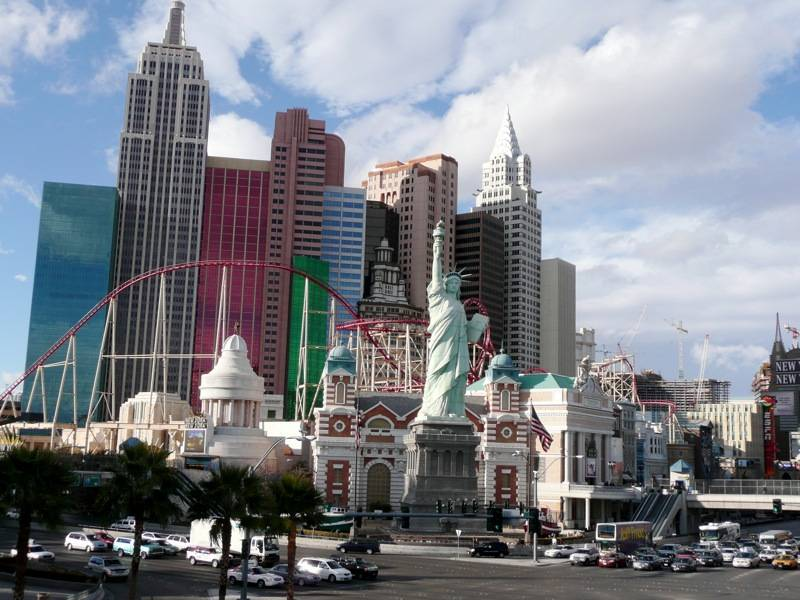
\includegraphics[width=0.75\linewidth, keepaspectratio=true]{placeholder/800-600-1}
    \caption{A sample figure of the New York Hotel at Las Vegas, NV, USA showing the effect of a loooong looooong caption.}
    \label{fig:sample-figure}
\end{figure}

\begin{figure}
    \centering
    \begin{subfigure}[b]{0.49\textwidth}
        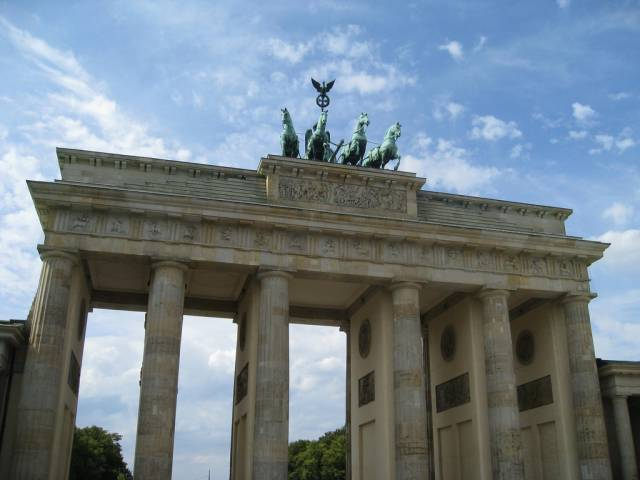
\includegraphics[width=\textwidth, keepaspectratio]{placeholder/640-480-1}
        \caption{Picture 1.}
        \label{fig:subfigures-two:1}
    \end{subfigure}
    \hfill
    \begin{subfigure}[b]{0.49\textwidth}
        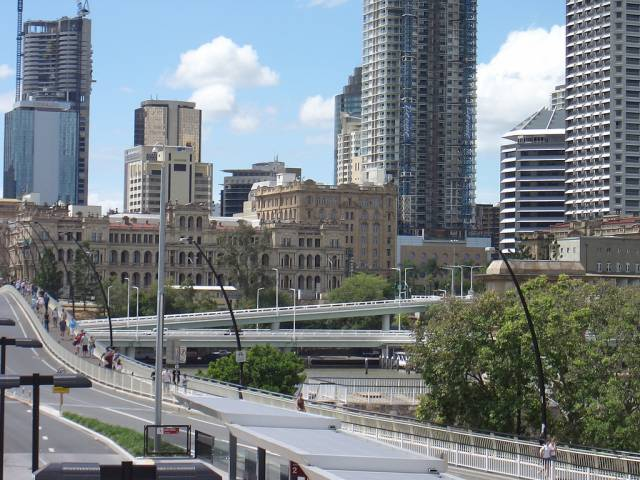
\includegraphics[width=\textwidth, keepaspectratio]{placeholder/640-480-2}
        \caption{Picture 2.}
        \label{fig:subfigures-two:2}
    \end{subfigure}
    
    \caption{Even subfigures of two figures are possible and the left one is referenced like \subref{fig:subfigures-two:1} so, while the right one is referenced like \subref{fig:subfigures-two:2} so.}
    \label{fig:subfigures-two}
\end{figure}

\begin{figure}
    \centering
    \begin{subfigure}[b]{0.49\textwidth}
        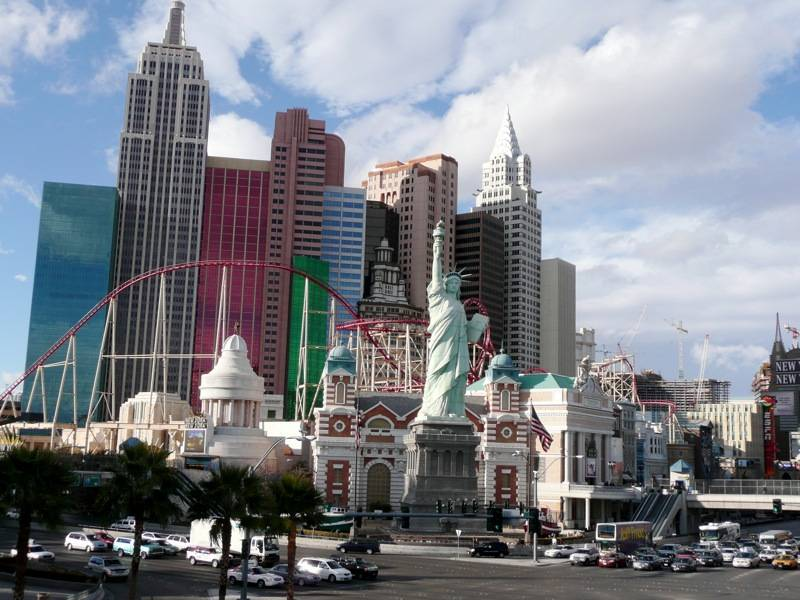
\includegraphics[width=\textwidth, keepaspectratio]{placeholder/800-600-1}
        \caption{Picture 1.}
        \label{fig:subfigures-four:1}
    \end{subfigure}
    \hfill
    \begin{subfigure}[b]{0.49\textwidth}
        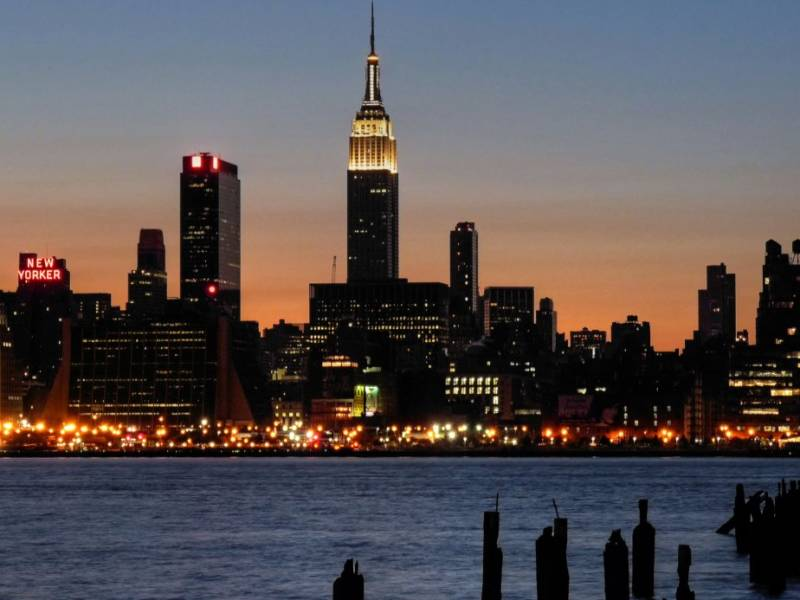
\includegraphics[width=\textwidth, keepaspectratio]{placeholder/800-600-2}
        \caption{Picture 2.}
        \label{fig:subfigures-four:2}
    \end{subfigure}
    \hfill
    \begin{subfigure}[b]{0.49\textwidth}
        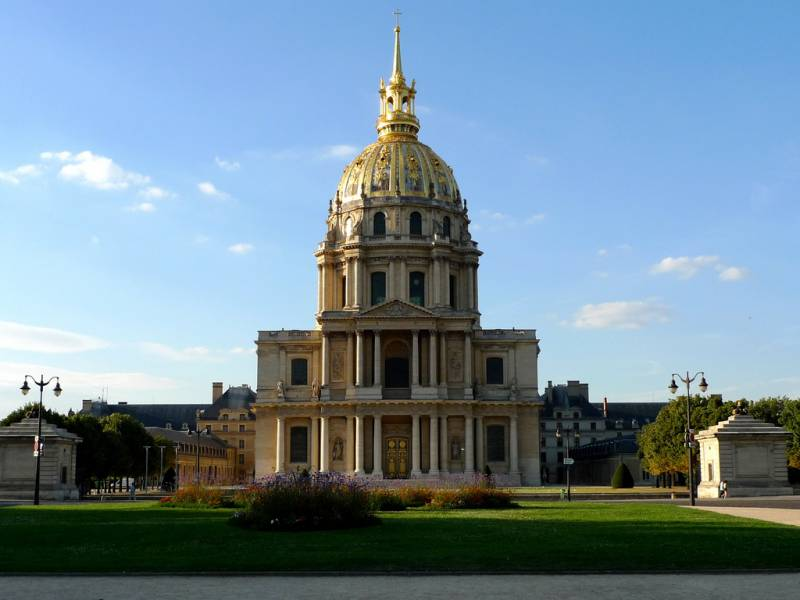
\includegraphics[width=\textwidth, keepaspectratio]{placeholder/800-600-3}
        \caption{Picture 3.}
        \label{fig:subfigures-four:3}
    \end{subfigure}
    \hfill
    \begin{subfigure}[b]{0.49\textwidth}
        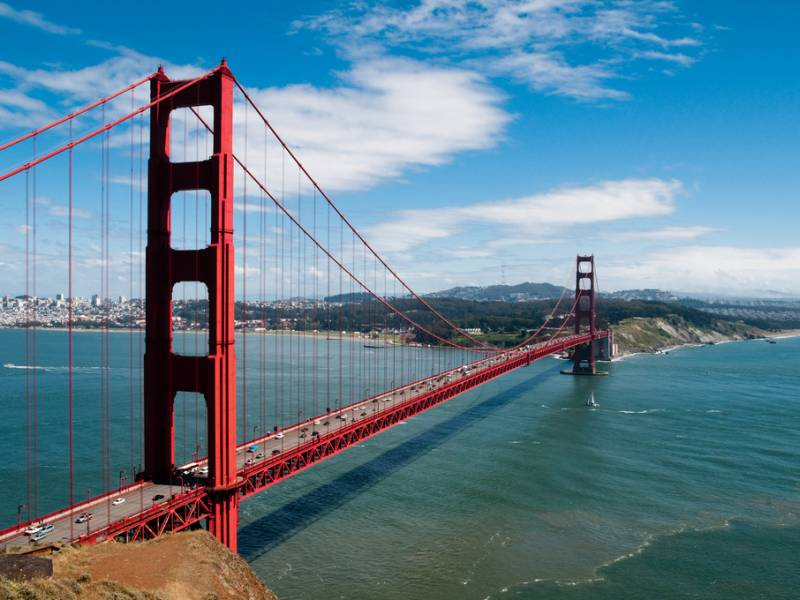
\includegraphics[width=\textwidth, keepaspectratio]{placeholder/800-600-4}
        \caption{Picture 4.}
        \label{fig:subfigures-four:4}
    \end{subfigure}
    
    \caption{Even subfigures of four figures are possible.}
    \label{fig:subfigures-four}
\end{figure}

\begin{table}
    \centering
    \caption{A sample table}
    \label{tbl:sample-table}
    \begin{tabular}{@{}llr@{}} \toprule
        \multicolumn{2}{c}{Item} \\ \cmidrule(r){1-2}
        Animal & Description & Price (\$)\\ \midrule
        Gnat  & per gram  & 13.65 \\
        & each      & 0.01 \\
        Gnu   & stuffed   & 92.50 \\
        Emu   & stuffed   & 33.33 \\
        Armadillo & frozen & 8.99 \\ \bottomrule
    \end{tabular}
\end{table}

\begin{table}
    \centering
    \caption{Tables can look nice, even for many many data to display}
    \label{tbl:sample-table-large}
    \begin{tabular}{SSSSSSSS} \toprule
        {$m$} & {$\Re\{\underline{\mathfrak{X}}(m)\}$} & {$-\Im\{\underline{\mathfrak{X}}(m)\}$} & {$\mathfrak{X}(m)$} & {$\frac{\mathfrak{X}(m)}{23}$} & {$A_m$} & {$\varphi(m)\ /\ ^{\circ}$} & {$\varphi_m\ /\ ^{\circ}$} \\ \midrule
        1  & 16.128 & +8.872 & 16.128 & 1.402 & 1.373 & -146.6 & -137.6 \\
        2  & 3.442  & -2.509 & 3.442  & 0.299 & 0.343 & 133.2  & 152.4  \\
        3  & 1.826  & -0.363 & 1.826  & 0.159 & 0.119 & 168.5  & -161.1 \\
        4  & 0.993  & -0.429 & 0.993  & 0.086 & 0.08  & 25.6   & 90     \\ \midrule
        5  & 1.29   & +0.099 & 1.29   & 0.112 & 0.097 & -175.6 & -114.7 \\
        6  & 0.483  & -0.183 & 0.483  & 0.042 & 0.063 & 22.3   & 122.5  \\
        7  & 0.766  & -0.475 & 0.766  & 0.067 & 0.039 & 141.6  & -122   \\
        8  & 0.624  & +0.365 & 0.624  & 0.054 & 0.04  & -35.7  & 90     \\ \midrule
        9  & 0.641  & -0.466 & 0.641  & 0.056 & 0.045 & 133.3  & -106.3 \\
        10 & 0.45   & +0.421 & 0.45   & 0.039 & 0.034 & -69.4  & 110.9  \\
        11 & 0.598  & -0.597 & 0.598  & 0.052 & 0.025 & 92.3   & -109.3 \\ \bottomrule
    \end{tabular}
\end{table}

%    \begin{lstlisting}
%        \begin{minted}{latex}
%\begin{figure}
%    \centering
%    \includegraphics[width=\linewidth, keepaspectratio=true]%
%        {placeholder/14942249547_f7f1d3e8bd_k}
%    \caption{A sample figure to show the effect of a loooong looooong caption. %
%        Credits by \url{https://www.flickr.com/photos/schubi74/14942249547/}.}
%    \label{fig:sample-figure}
%\end{figure}
%        \end{minted}
%        \caption{Sample code for \cref{fig:sample-figure}}
%        \label{lst:sample-code}
%    \end{lstlisting}

For figures, the guidelines are:

\begin{itemize}
    \item Always center images using \lstinline!\centering! as the very first command of the \lstinline!figure!-environment.
    \item Make sure to set the width of your included images explicitely using the \lstinline!width=! option. Have a single figure's width set to \lstinline!width=0.75\linewidth!, while two figures side by side must be set to \lstinline!width=\linewidth! as long as you set the width of the surrounding \lstinline!minipage! or \lstinline!subfigure! to \lstinline!0.49\linewidth!.
    \item Don't forget to keep the aspect ratio of images if you change their width.
    \item Never ever under sample images. In other words: never ever enlarge images.
    \item It's best to use vector graphics i.e., \lstinline!*.eps! or \lstinline!*.tikz! for proper quality in both PDFs as well as on screen.
    \item Add a caption to your image. Captions must be below the image.
    \item Let the labels be handled automatically by \LaTeX. A best practice is to set the prefix of figures' labels to \lstinline!fig:!.
    \item For a good example see \cref{fig:sample-figure} and its code at \cref{lst:sample-code} (this reference was created using the \lstinline!\cref{}! command).
    \item Always add a full stop to your figure captions like so.
    \item Do not be afraid to use lengthy figure and table captions-—better that than confusing or incomplete ones.
    \item Figure and table captions must be elaborative i.e., do not fear having captions that span multiple lines. No really, don't.
    \item If your table or figure caption is too long in the list of figures or list of tables, respectively, use the short-caption option to \lstinline!\caption! which looks like \lstinline!\caption[This short caption shows up in the list of figures/tables]{While this very long long caption actually shows up under the caption just to show that it would be too long and spans multiple lines in the list of figures/tables.}!.
    \item If your figure or table is essentially the same as or based on another author’s, but you recreated or adapted it, it is standard to include the words ``Adapted from'' or ``After'' followed by the author’s name and a citation at the end of the caption.
    \item Always cite the figure or table if it—--or its data—--came from a source, using the same citation style that you have used throughout the paper. The most logical place for the citation to appear is at the end of the caption. See \cref{sec:referencing} of this manual for a thorough discussion of rules for source citation.
    \item Do not crowd a table or figure, neither within itself nor within your text; give it room to breathe. When it appears amidst your body text, skip at least one line above and below it.
    \item Rule of thumb: Try to present the table or figure so that it would make sense even if ripped from the paper.
    \item If possible, label the axes of graphs with full words: ``Temperature versus time'' rather than ``T versus t.''
    \item Be certain that your legend—--that part of the figure where you define any symbols or other visual markers that appear—--is readable, clear, and meaningfully placed. As long as it does not overwhelm the rest of the figure, do not be afraid to make the legend large to enhance its readability.
    \item Use footnotes (a simple asterisk to indicate them will do) for explanatory material such as the number of respondents to a survey or the fact that certain values were estimated.
\end{itemize}

For tables, the guidelines are

\begin{itemize}
    \item The legend (sometimes called the caption) goes above the Table.
    \item Units are specified in column headings wherever appropriate.
    \item Lines of demarcation are used to set legend, headers, data, and footnotes apart from one another.
    \item Footnotes are used to clarify points in the table, or to convey repetitive information about entries.
    \item Footnotes may also be used to denote statistical differences among groups.
\end{itemize}


\section{Coloring}

There are a few basic colors that are set for some default coloring of tables and should be used primarily for other things, where applicable.
For all the available color commands and a sample of the rendered color, please see \cref{tbl:color-samples}.

\begin{table}
    \centering
    \caption{List of available color codes and a sample colored box}
    \label{tbl:color-samples}
    \begin{tabular}{ll} \toprule
        Color Code
            & Color Sample \\ \midrule
        MainColorVeryLight
            & \crule[MainColorVeryLight]{7.5cm}{1cm} \\
        MainColorLight
            & \crule[MainColorLight]{7.5cm}{1cm} \\
        MainColor
            & \crule[MainColor]{7.5cm}{1cm} \\
        MainColorDark
            & \crule[MainColorDark]{7.5cm}{1cm} \\
        MainColorVeryDark
            & \crule[MainColorVeryDark]{7.5cm}{1cm} \\
        PrimaryColorVeryLight
            & \crule[PrimaryColorVeryLight]{7.5cm}{1cm} \\
        PrimaryColorLight
            & \crule[PrimaryColorLight]{7.5cm}{1cm} \\
        PrimaryColor
            & \crule[PrimaryColor]{7.5cm}{1cm} \\
        PrimaryColorDark
            & \crule[PrimaryColorDark]{7.5cm}{1cm} \\
        PrimaryColorVeryDark
            & \crule[PrimaryColorVeryDark]{7.5cm}{1cm} \\
        SecondaryColorVeryLight
            & \crule[SecondaryColorVeryLight]{7.5cm}{1cm} \\
        SecondaryColorLight
            & \crule[SecondaryColorLight]{7.5cm}{1cm} \\
        SecondaryColor
            & \crule[SecondaryColor]{7.5cm}{1cm} \\
        SecondaryColorDark
            & \crule[SecondaryColorDark]{7.5cm}{1cm} \\
        SecondaryColorVeryDark
            & \crule[SecondaryColorVeryDark]{7.5cm}{1cm} \\ \bottomrule
    \end{tabular}
\end{table}



\section{Referencing}\label{sec:referencing}

Referencing may be done using \lstinline!\ref{label}! even though usage of \lstinline!\cref{label}! is encouraged for that it automatically typesets the appropriate type like \texttt{Eqn.} or \texttt{Fig.}, \texttt{Tbl.}, or \texttt{Listing} to whatever is being reference. At the beginning of a sentence, \lstinline!\Cref{label}! must be used to fully give the referenced type in words. \Cref{fig:sample-figure} refers to a sample figure at the beginning of a sentence, while \cref{fig:sample-figure} refers to a sample figure in text.

\begin{itemize}
    \item Capitalize and write in words the reference object at the beginning of a sentence.
    \item Otherwise use the abbreviated forms of \texttt{Fig.}, \texttt{Eqn.}, and \texttt{Tbl.} for referencing figures, equations, and tables, respectively.
    \item Refer to the \lstinline!cleveref! package documentation at \\\url{http://www.ctan.org/pkg/cleveref}.
\end{itemize}

\subsection{Subsection}

\subsubsection{Subsubsection}

\paragraph{Paragraph}

\subparagraph{Subparagraph}
    
    %% Last but not least the bilbiography
    \bibliography{demo/bibliography.bib}
    
    %% After the main content, you might want to add some appendices (like source code
    % or more detailed derivations of equations)
    % @todo The "\part{Appendices}" needs some adjustment in its style
    \begin{appendices}
        \chapter{Some Lengthy Mathematical Equations}
\section{First Section of Appendix One}
\section{Second Section of Appendix One}

\chapter{Some Lengthy Source Code Listings}
\section{First Section of Appendix Two}
\section{Second Section of Appendix Two}
\section{Third Section of Appendix Two}
    \end{appendices}
    
\end{document}